\documentclass{article}

\def \lastexercisenumber{6}

% Hier befinden sich Pakete, die wir beinahe immer benutzen ...

\usepackage[utf8]{inputenc}

% Sprach-Paket:
\usepackage[ngerman]{babel}

% damit's nicht so, wie beim Grill aussieht:
\usepackage{fullpage}

% Mathematik:
\usepackage{amsmath, amssymb, amsfonts, amsthm}
\usepackage{bbm}
\usepackage{mathtools, mathdots}

% Makros mit mehereren Default-Argumenten:
\usepackage{twoopt}

% Anführungszeichen (Makro \Quote{}):
\usepackage{babel}

% if's für Makros:
\usepackage{xifthen}
\usepackage{etoolbox}

% tikz ist kein Zeichenprogramm (doch!):
\usepackage{tikz}

% bessere Aufzählungen:
\usepackage{enumitem}

% (bessere) Umgebung für Bilder:
\usepackage{graphicx, subfig, float}

% Umgebung für Code:
\usepackage{listings}

% Farben:
\usepackage{xcolor}

% Umgebung für "plain text":
\usepackage{verbatim}

% Umgebung für mehrerer Spalten:
\usepackage{multicol}

% "nette" Brüche
\usepackage{nicefrac}

% Spaltentypen verschiedener Dicke
\usepackage{tabularx}
\usepackage{makecell}

% Für Vektoren
\usepackage{esvect}

% (Web-)Links
\usepackage{hyperref}

% Zitieren & Literatur-Verzeichnis
\usepackage[style = authoryear]{biblatex}
\usepackage{csquotes}

% so ähnlich wie mathbb
%\usepackage{mathds}

% Keine Ahnung, was das macht ...
\usepackage{booktabs}
\usepackage{ngerman}
\usepackage{placeins}

% special letters:

\newcommand{\N}{\mathbb{N}}
\newcommand{\Z}{\mathbb{Z}}
\newcommand{\Q}{\mathbb{Q}}
\newcommand{\R}{\mathbb{R}}
\newcommand{\C}{\mathbb{C}}
\newcommand{\K}{\mathbb{K}}
\newcommand{\T}{\mathbb{T}}
\newcommand{\E}{\mathbb{E}}
\newcommand{\V}{\mathbb{V}}
\renewcommand{\S}{\mathbb{S}}
\renewcommand{\P}{\mathbb{P}}
\newcommand{\1}{\mathbbm{1}}

% quantors:

\newcommand{\Forall}{\forall \,}
\newcommand{\Exists}{\exists \,}
\newcommand{\ExistsOnlyOne}{\exists! \,}
\newcommand{\nExists}{\nexists \,}
\newcommand{\ForAlmostAll}{\forall^\infty \,}

% MISC symbols:

\newcommand{\landau}{{\scriptstyle \mathcal{O}}}
\newcommand{\Landau}{\mathcal{O}}


\newcommand{\eps}{\mathrm{eps}}

% graphics in a box:

\newcommandtwoopt
{\includegraphicsboxed}[3][][]
{
  \begin{figure}[!h]
    \begin{boxedin}
      \ifthenelse{\isempty{#1}}
      {
        \begin{center}
          \includegraphics[width = 0.75 \textwidth]{#3}
          \label{fig:#2}
        \end{center}
      }{
        \begin{center}
          \includegraphics[width = 0.75 \textwidth]{#3}
          \caption{#1}
          \label{fig:#2}
        \end{center}
      }
    \end{boxedin}
  \end{figure}
}

% braces:

\newcommand{\pbraces}[1]{{\left  ( #1 \right  )}}
\newcommand{\bbraces}[1]{{\left  [ #1 \right  ]}}
\newcommand{\Bbraces}[1]{{\left \{ #1 \right \}}}
\newcommand{\vbraces}[1]{{\left  | #1 \right  |}}
\newcommand{\Vbraces}[1]{{\left \| #1 \right \|}}
\newcommand{\abraces}[1]{{\left \langle #1 \right \rangle}}
\newcommand{\round}[1]{\bbraces{#1}}

\newcommand
{\floorbraces}[1]
{{\left \lfloor #1 \right \rfloor}}

\newcommand
{\ceilbraces} [1]
{{\left \lceil  #1 \right \rceil }}

% special functions:

\newcommand{\norm}  [2][]{\Vbraces{#2}_{#1}}
\newcommand{\diam}  [2][]{\mathrm{diam}_{#1} \: #2}
\newcommand{\diag}  [1]{\mathrm{diag} \: #1}
\newcommand{\dist}  [1]{\mathrm{dist} \: #1}
\newcommand{\mean}  [1]{\mathrm{mean} \: #1}
\newcommand{\erf}   [1]{\mathrm{erf} \: #1}
\newcommand{\id}    [1]{\mathrm{id} \: #1}
\newcommand{\sgn}   [1]{\mathrm{sgn} \: #1}
\newcommand{\supp}  [1]{\mathrm{supp} \: #1}
\newcommand{\arsinh}[1]{\mathrm{arsinh} \: #1}
\newcommand{\arcosh}[1]{\mathrm{arcosh} \: #1}
\newcommand{\artanh}[1]{\mathrm{artanh} \: #1}
\newcommand{\card}  [1]{\mathrm{card} \: #1}
\newcommand{\Span}  [1]{\mathrm{span} \: #1}
\newcommand{\Aut}   [1]{\mathrm{Aut} \: #1}
\newcommand{\End}   [1]{\mathrm{End} \: #1}
\newcommand{\ggT}   [1]{\mathrm{ggT} \: #1}
\newcommand{\kgV}   [1]{\mathrm{kgV} \: #1}
\newcommand{\ord}   [1]{\mathrm{ord} \: #1}
\newcommand{\grad}  [1]{\mathrm{grad} \: #1}
\newcommand{\ran}   [1]{\mathrm{ran} \: #1}
\newcommand{\graph} [1]{\mathrm{graph} \: #1}
\newcommand{\Inv}   [1]{\mathrm{Inv} \: #1}
\newcommand{\pv}    [1]{\mathrm{pv} \: #1}
\newcommand{\GL}    [1]{\mathrm{GL} \: #1}
\newcommand{\Mod}{\mathrm{Mod} \:}
\newcommand{\Th}{\mathrm{Th} \:}
\newcommand{\Char}{\mathrm{char}}
\newcommand{\At}{\mathrm{At}}
\newcommand{\Ob}{\mathrm{Ob}}
\newcommand{\Hom}{\mathrm{Hom}}
\newcommand{\orthogonal}[3][]{#2 ~\bot_{#1}~ #3}
\newcommand{\Rang}{\mathrm{Rang}}
\newcommand{\NIL}{\mathrm{NIL}}
\newcommand{\Res}{\mathrm{Res}}
\newcommand{\lxor}{\dot \lor}
\newcommand{\Div}{\mathrm{div} \:}
\newcommand{\meas}{\mathrm{meas} \:}

% fractions:

\newcommand{\Frac}[2]{\frac{1}{#1} \pbraces{#2}}
\newcommand{\nfrac}[2]{\nicefrac{#1}{#2}}

% derivatives & integrals:

\newcommandtwoopt
{\Int}[4][][]
{\int_{#1}^{#2} #3 ~\mathrm{d} #4}

\newcommandtwoopt
{\derivative}[3][][]
{
  \frac
  {\mathrm{d}^{#1} #2}
  {\mathrm{d} #3^{#1}}
}

\newcommandtwoopt
{\pderivative}[3][][]
{
  \frac
  {\partial^{#1} #2}
  {\partial #3^{#1}}
}

\newcommand
{\primeprime}
{{\prime \prime}}

\newcommand
{\primeprimeprime}
{{\prime \prime \prime}}

% Text:

\newcommand{\Quote}[1]{\glqq #1\grqq{}}
\newcommand{\Text}[1]{{\text{#1}}}
\newcommand{\fastueberall}{\text{f.ü.}}
\newcommand{\fastsicher}{\text{f.s.}}

% -------------------------------- %
% amsthm-stuff:

\theoremstyle{definition}

% numbered theorems
\newtheorem{theorem}{Satz}
\newtheorem{lemma}{Lemma}
\newtheorem{corollary}{Korollar}
\newtheorem{proposition}{Proposition}
\newtheorem{remark}{Bemerkung}
\newtheorem{definition}{Definition}
\newtheorem{example}{Beispiel}

% unnumbered theorems
\newtheorem*{theorem*}{Satz}
\newtheorem*{lemma*}{Lemma}
\newtheorem*{corollary*}{Korollar}
\newtheorem*{proposition*}{Proposition}
\newtheorem*{remark*}{Bemerkung}
\newtheorem*{definition*}{Definition}
\newtheorem*{example*}{Beispiel}

% Please define this stuff in project ("main.tex"):

% \def \lastexercisenumber {...}
% This will be 0 by default

% \setcounter{section}{...}
% This will be 0 by default
% and hence, completely ignored

\ifnum \thesection = 0
{\newtheorem{exercise}{Aufgabe}}
\else
{\newtheorem{exercise}{Aufgabe}[section]}
\fi

\ifdef
{\lastexercisenumber}
{\setcounter{exercise}{\lastexercisenumber}}

\newcommand{\solution}
{
    \renewcommand{\proofname}{Lösung}
    \renewcommand{\qedsymbol}{}
    \proof
}

\renewcommand{\proofname}{Beweis}

% -------------------------------- %
% environment zum einkasteln:

% dickere vertical lines
\newcolumntype
{x}
[1]
{!{\centering\arraybackslash\vrule width #1}}

% environment selbst (the big cheese)
\newenvironment
{boxedin}
{
  \begin{tabular}
  {
    x{1 pt}
    p{\textwidth}
    x{1 pt}
  }
  \Xhline
  {2 \arrayrulewidth}
}
{
  \\
  \Xhline{2 \arrayrulewidth}
  \end{tabular}
}

% -------------------------------- %
% MISC "Ein-Deutschungen"

\renewcommand
{\figurename}
{Abbildung}

\renewcommand
{\tablename}
{Tabelle}

% -------------------------------- %

% ---------------------------------------------------------------- %
% https://www.overleaf.com/learn/latex/Code_listing

\definecolor{codegreen} {rgb}{0, 0.6, 0}
\definecolor{codegray}    {rgb}{0.5, 0.5, 0.5}
\definecolor{codepurple}{rgb}{0.58, 0, 0.82}
\definecolor{backcolour}{rgb}{0.95, 0.95, 0.92}

\lstdefinestyle{overleaf}
{
    backgroundcolor = \color{backcolour},
    commentstyle = \color{codegreen},
    keywordstyle = \color{magenta},
    numberstyle = \tiny\color{codegray},
    stringstyle = \color{codepurple},
    basicstyle = \ttfamily \footnotesize,
    breakatwhitespace = false,
    breaklines = true,
    captionpos = b,
    keepspaces = true,
    numbers = left,
    numbersep = 5pt,
    showspaces = false,
    showstringspaces = false,
    showtabs = false,
    tabsize = 2
}

% ---------------------------------------------------------------- %
% https://en.wikibooks.org/wiki/LaTeX/Source_Code_Listings

\lstdefinestyle{customc}
{
    belowcaptionskip = 1 \baselineskip,
    breaklines = true,
    frame = L,
    xleftmargin = \parindent,
    language = C,
    showstringspaces = false,
    basicstyle = \footnotesize \ttfamily,
    keywordstyle = \bfseries \color{green!40!black},
    commentstyle = \itshape \color{purple!40!black},
    identifierstyle = \color{blue},
    stringstyle = \color{orange},
}

\lstdefinestyle{customasm}
{
    belowcaptionskip = 1 \baselineskip,
    frame = L,
    xleftmargin = \parindent,
    language = [x86masm] Assembler,
    basicstyle = \footnotesize\ttfamily,
    commentstyle = \itshape\color{purple!40!black},
}

% ---------------------------------------------------------------- %
% https://tex.stackexchange.com/questions/235731/listings-syntax-for-literate

\definecolor{maroon}        {cmyk}{0, 0.87, 0.68, 0.32}
\definecolor{halfgray}      {gray}{0.55}
\definecolor{ipython_frame} {RGB}{207, 207, 207}
\definecolor{ipython_bg}    {RGB}{247, 247, 247}
\definecolor{ipython_red}   {RGB}{186, 33, 33}
\definecolor{ipython_green} {RGB}{0, 128, 0}
\definecolor{ipython_cyan}  {RGB}{64, 128, 128}
\definecolor{ipython_purple}{RGB}{170, 34, 255}

\lstdefinestyle{stackexchangePython}
{
    breaklines = true,
    %
    extendedchars = true,
    literate =
    {á}{{\' a}} 1 {é}{{\' e}} 1 {í}{{\' i}} 1 {ó}{{\' o}} 1 {ú}{{\' u}} 1
    {Á}{{\' A}} 1 {É}{{\' E}} 1 {Í}{{\' I}} 1 {Ó}{{\' O}} 1 {Ú}{{\' U}} 1
    {à}{{\` a}} 1 {è}{{\` e}} 1 {ì}{{\` i}} 1 {ò}{{\` o}} 1 {ù}{{\` u}} 1
    {À}{{\` A}} 1 {È}{{\' E}} 1 {Ì}{{\` I}} 1 {Ò}{{\` O}} 1 {Ù}{{\` U}} 1
    {ä}{{\" a}} 1 {ë}{{\" e}} 1 {ï}{{\" i}} 1 {ö}{{\" o}} 1 {ü}{{\" u}} 1
    {Ä}{{\" A}} 1 {Ë}{{\" E}} 1 {Ï}{{\" I}} 1 {Ö}{{\" O}} 1 {Ü}{{\" U}} 1
    {â}{{\^ a}} 1 {ê}{{\^ e}} 1 {î}{{\^ i}} 1 {ô}{{\^ o}} 1 {û}{{\^ u}} 1
    {Â}{{\^ A}} 1 {Ê}{{\^ E}} 1 {Î}{{\^ I}} 1 {Ô}{{\^ O}} 1 {Û}{{\^ U}} 1
    {œ}{{\oe}}  1 {Œ}{{\OE}}  1 {æ}{{\ae}}  1 {Æ}{{\AE}}  1 {ß}{{\ss}}  1
    {ç}{{\c c}} 1 {Ç}{{\c C}} 1 {ø}{{\o}} 1 {å}{{\r a}} 1 {Å}{{\r A}} 1
    {€}{{\EUR}} 1 {£}{{\pounds}} 1
}


% Python definition (c) 1998 Michael Weber
% Additional definitions (2013) Alexis Dimitriadis
% modified by me (should not have empty lines)

\lstdefinelanguage{iPython}{
    morekeywords = {access, and, break, class, continue, def, del, elif, else, except, exec, finally, for, from, global, if, import, in, is, lambda, not, or, pass, print, raise, return, try, while}, %
    %
    % Built-ins
    morekeywords = [2]{abs, all, any, basestring, bin, bool, bytearray, callable, chr, classmethod, cmp, compile, complex, delattr, dict, dir, divmod, enumerate, eval, execfile, file, filter, float, format, frozenset, getattr, globals, hasattr, hash, help, hex, id, input, int, isinstance, issubclass, iter, len, list, locals, long, map, max, memoryview, min, next, object, oct, open, ord, pow, property, range, raw_input, reduce, reload, repr, reversed, round, set, setattr, slice, sorted, staticmethod, str, sum, super, tuple, type, unichr, unicode, vars, xrange, zip, apply, buffer, coerce, intern}, %
    %
    sensitive = true, %
    morecomment = [l] \#, %
    morestring = [b]', %
    morestring = [b]", %
    %
    morestring = [s]{'''}{'''}, % used for documentation text (mulitiline strings)
    morestring = [s]{"""}{"""}, % added by Philipp Matthias Hahn
    %
    morestring = [s]{r'}{'},     % `raw' strings
    morestring = [s]{r"}{"},     %
    morestring = [s]{r'''}{'''}, %
    morestring = [s]{r"""}{"""}, %
    morestring = [s]{u'}{'},     % unicode strings
    morestring = [s]{u"}{"},     %
    morestring = [s]{u'''}{'''}, %
    morestring = [s]{u"""}{"""}, %
    %
    % {replace}{replacement}{lenght of replace}
    % *{-}{-}{1} will not replace in comments and so on
    literate = 
    {á}{{\' a}} 1 {é}{{\' e}} 1 {í}{{\' i}} 1 {ó}{{\' o}} 1 {ú}{{\' u}} 1
    {Á}{{\' A}} 1 {É}{{\' E}} 1 {Í}{{\' I}} 1 {Ó}{{\' O}} 1 {Ú}{{\' U}} 1
    {à}{{\` a}} 1 {è}{{\` e}} 1 {ì}{{\` i}} 1 {ò}{{\` o}} 1 {ù}{{\` u}} 1
    {À}{{\` A}} 1 {È}{{\' E}} 1 {Ì}{{\` I}} 1 {Ò}{{\` O}} 1 {Ù}{{\` U}} 1
    {ä}{{\" a}} 1 {ë}{{\" e}} 1 {ï}{{\" i}} 1 {ö}{{\" o}} 1 {ü}{{\" u}} 1
    {Ä}{{\" A}} 1 {Ë}{{\" E}} 1 {Ï}{{\" I}} 1 {Ö}{{\" O}} 1 {Ü}{{\" U}} 1
    {â}{{\^ a}} 1 {ê}{{\^ e}} 1 {î}{{\^ i}} 1 {ô}{{\^ o}} 1 {û}{{\^ u}} 1
    {Â}{{\^ A}} 1 {Ê}{{\^ E}} 1 {Î}{{\^ I}} 1 {Ô}{{\^ O}} 1 {Û}{{\^ U}} 1
    {œ}{{\oe}}  1 {Œ}{{\OE}}  1 {æ}{{\ae}}  1 {Æ}{{\AE}}  1 {ß}{{\ss}}  1
    {ç}{{\c c}} 1 {Ç}{{\c C}} 1 {ø}{{\o}} 1 {å}{{\r a}} 1 {Å}{{\r A}} 1
    {€}{{\EUR}} 1 {£}{{\pounds}} 1
    %
    {^}{{{\color{ipython_purple}\^ {}}}} 1
    { = }{{{\color{ipython_purple} = }}} 1
    %
    {+}{{{\color{ipython_purple}+}}} 1
    {*}{{{\color{ipython_purple}$^\ast$}}} 1
    {/}{{{\color{ipython_purple}/}}} 1
    %
    {+=}{{{+=}}} 1
    {-=}{{{-=}}} 1
    {*=}{{{$^\ast$ = }}} 1
    {/=}{{{/=}}} 1,
    literate = 
    *{-}{{{\color{ipython_purple} -}}} 1
     {?}{{{\color{ipython_purple} ?}}} 1,
    %
    identifierstyle = \color{black}\ttfamily,
    commentstyle = \color{ipython_cyan}\ttfamily,
    stringstyle = \color{ipython_red}\ttfamily,
    keepspaces = true,
    showspaces = false,
    showstringspaces = false,
    %
    rulecolor = \color{ipython_frame},
    frame = single,
    frameround = {t}{t}{t}{t},
    framexleftmargin = 6mm,
    numbers = left,
    numberstyle = \tiny\color{halfgray},
    %
    %
    backgroundcolor = \color{ipython_bg},
    % extendedchars = true,
    basicstyle = \scriptsize,
    keywordstyle = \color{ipython_green}\ttfamily,
}

% ---------------------------------------------------------------- %
% https://tex.stackexchange.com/questions/417884/colour-r-code-to-match-knitr-theme-using-listings-minted-or-other

\geometry{verbose, tmargin = 2.5cm, bmargin = 2.5cm, lmargin = 2.5cm, rmargin = 2.5cm}

\definecolor{backgroundCol}  {rgb}{.97, .97, .97}
\definecolor{commentstyleCol}{rgb}{0.678, 0.584, 0.686}
\definecolor{keywordstyleCol}{rgb}{0.737, 0.353, 0.396}
\definecolor{stringstyleCol} {rgb}{0.192, 0.494, 0.8}
\definecolor{NumCol}         {rgb}{0.686, 0.059, 0.569}
\definecolor{basicstyleCol}  {rgb}{0.345, 0.345, 0.345}

\lstdefinestyle{stackexchangeR}
{
    language = R,                                        % the language of the code
    basicstyle = \small \ttfamily \color{basicstyleCol}, % the size of the fonts that are used for the code
    % numbers = left,                                      % where to put the line-numbers
    numberstyle = \color{green},                         % the style that is used for the line-numbers
    stepnumber = 1,                                      % the step between two line-numbers. If it is 1, each line will be numbered
    numbersep = 5pt,                                     % how far the line-numbers are from the code
    backgroundcolor = \color{backgroundCol},             % choose the background color. You must add \usepackage{color}
    showspaces = false,                                  % show spaces adding particular underscores
    showstringspaces = false,                            % underline spaces within strings
    showtabs = false,                                    % show tabs within strings adding particular underscores
    % frame = single,                                      % adds a frame around the code
    % rulecolor = \color{white},                           % if not set, the frame-color may be changed on line-breaks within not-black text (e.g. commens (green here))
    tabsize = 2,                                         % sets default tabsize to 2 spaces
    captionpos = b,                                      % sets the caption-position to bottom
    breaklines = true,                                   % sets automatic line breaking
    breakatwhitespace = false,                           % sets if automatic breaks should only happen at whitespace
    keywordstyle = \color{keywordstyleCol},              % keyword style
    commentstyle = \color{commentstyleCol},              % comment style
    stringstyle = \color{stringstyleCol},                % string literal style
    literate = %
    *{0}{{{\color{NumCol} 0}}} 1
     {1}{{{\color{NumCol} 1}}} 1
     {2}{{{\color{NumCol} 2}}} 1
     {3}{{{\color{NumCol} 3}}} 1
     {4}{{{\color{NumCol} 4}}} 1
     {5}{{{\color{NumCol} 5}}} 1
     {6}{{{\color{NumCol} 6}}} 1
     {7}{{{\color{NumCol} 7}}} 1
     {8}{{{\color{NumCol} 8}}} 1
     {9}{{{\color{NumCol} 9}}} 1
}

% ---------------------------------------------------------------- %
% Fundament Mathematik

\lstdefinestyle{fundament}{basicstyle = \ttfamily}

% ---------------------------------------------------------------- %


\parskip 0pt
\parindent 0pt

\title
{
  Diskrete und Geometrische Algorithmen \\
  \vspace{4pt}
  \normalsize
  \textit{2. Übung am 19.10.2020}
}
\author
{
  Richard Weiss
  \and
  Florian Schager
  \and
  Christian Sallinger
  \and
  Fabian Zehetgruber
  \and
  Paul Winkler
  \and
  Christian Göth
}
\date{}

\begin{document}

\maketitle

% --------------------------------------------------------------------------------

\begin{exercise}

Zum asymptotischen Vergleich von Folgen:

\begin{enumerate}[label = (\alph*)]

  \item Vergleichen Sie das asymptotische Verhalten von $f(n) = n!$ und $g(n) = (n + 2)!$, also überlegen Sie sich ob eine (welche) der Funktionen ein $\landau, \Landau, \omega, \Omega, \Theta$ der anderen Funktion ist.

  \item Vergleichen Sie das asymptotische Verhalten von $f(n) = n^{\log_2(4)}$ und $g(n) = 3^{\log_2(n)}$, also überlegen Sie sich ob eine (welche) der Funktionen ein $\landau, \Landau, \omega, \Omega, \Theta$ der anderen Funktion ist.

  \item Zeigen Sie an Hand der Defintion, dass für positive Funktionen $f$ und $g$ die Beziehung

  \begin{align*}
    \max \Bbraces{f(n), g(n)} = \Theta(f(n) + g(n))
  \end{align*}

  gilt.

  \item Gilt selbige Beziehung ebenfalls für $\min \Bbraces{f(n), g(n)}$?

  \item Folgt aus $f(n) = \Landau(g(n))$, dass $2^{f(n)} = \Landau(2^{g(n)})$?

  \item Gilt für alle positiven Funktionen $f$ die Beziehung $f(n) = \Landau(f(n)^2)$?

  \item Finden Sie eine Funktion $f$, sodass weder $f(n) = \Landau(n)$ noch $f(n) = \Omega(n)$ gilt.

\end{enumerate}

\end{exercise}

% --------------------------------------------------------------------------------

\begin{solution}

\phantom{}

\begin{comment}

\includegraphicsboxed{Definition 1-4.png}
\includegraphicsboxed{Definition 1-5.png}
\includegraphicsboxed{Lemma 1-2.png}
\includegraphicsboxed{Lemma 1-3.png}

\end{comment}

\begin{enumerate}[label = (\alph*)]

  \item

  \begin{align*}
    \frac{f(n)}{g(n)} = \frac{n!}{(n+1)!} = \frac{1}{(n+2)(n+1)} \xrightarrow{n \to \infty} 0 \\
  \end{align*}

  \begin{align*}
    \stackrel{1.3.7}{\iff}
    f \in \landau(g)
    \stackrel{1.3.1}{\subseteq}
    \Landau(g) \\
    \stackrel{1.3.5}{\iff}
    g \in \omega(f)
    \stackrel{1.3.1}{\subseteq}
    \Omega(f)
  \end{align*}

  \begin{align*}
    \implies
    \frac{g(n)}{f(n)} \xrightarrow{n \to \infty} \infty
  \end{align*}

  \begin{align*}
    \stackrel{1.2.3}{\iff}
    g \not \in \Landau(f)
    \stackrel{1.3.2}{\supseteq}
    \landau(f) \\
    \stackrel{1.2.2}{\iff}
    f \not \in \Omega(g)
    \stackrel{1.3.2}{\supseteq}
    \omega(g)
  \end{align*}

  \begin{align*}
    \implies
    g
    \not \in
    \Landau(f) \cap \Omega(f)
    \stackrel{2.1.1}{=}
    \Theta(f) \\
    \implies
    f
    \not \in
    \Landau(g) \cap \Omega(g)
    \stackrel{2.1.1}{=}
    \Theta(g)
  \end{align*}

  \item

  \begin{align*}
    \log_2{4}               & = \log_2{2^2} = 2 \\
    \log_2{n}               & = \frac{\log_3{n}}{\log_3{2}} \\
    2 - \frac{1}{\log_3{2}} & > 0 \iff 2 > \frac{1}{\log_3{2}} \iff \log_3{4} = \log_3{2^2} = 2 \log_3{2} > 1 = \log_3{3^1}
  \end{align*}

  \begin{align*}
    \implies
    \frac{f(n)}{g(n)}
    =
    \frac{n^{\log_2{4}}}{3^{\log_2{n}}}
    =
    n^2 / \pbraces{3^{\log_3{n}}}^{1 / \log_3{2}}
    =
    n^{2 - \frac{1}{\log_3{2}}}
    \xrightarrow{n \to \infty} \infty
    \implies
    \frac{g(n)}{f(n)}
    \xrightarrow{n \to \infty} 0
  \end{align*}

  (b) ist also (a), verkehrt rum.

  \item

  \begin{comment}

    \begin{figure}[h!]
    \begin{boxedin}
      \vspace{0.5 cm}
      \hspace{0.5 cm}
      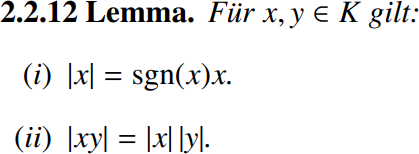
\includegraphics[width = 5 cm]{Kaltenbaeck - Fundament Analysis - Lemma 2-2-12-1.png} \\
      \vspace{0.01 cm}
      \hspace{0.5 cm}
      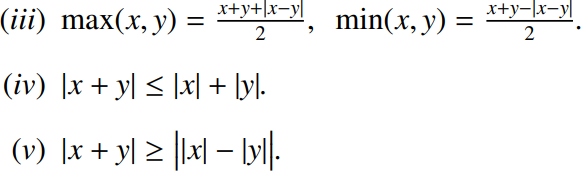
\includegraphics[width = 7 cm]{Kaltenbaeck - Fundament Analysis - Lemma 2-2-12-2.png} \\
      \vspace{0.5 cm}
      \caption{Kaltenbaeck - Fundament Analysis}
      \label{fig:KFAL2.2.12}
    \end{boxedin}
  \end{figure}

  \end{comment}

  Seien $c := 1/2$ und $d := 1$, dann gilt $\ForAlmostAll n \in \N:$

  \begin{multline*}
    c (f(n) + g(n))
    \leq
    \max \Bbraces{f(n), g(n)}
    =
    \frac{f(n) + g(n) + |f(n) - g(n)|}{2} \\
    \leq
    \frac{f(n) + g(n)}{2}
    +
    \frac{f(n) + g(n)}{2}
    =
    d (f(n) + g(n)).
  \end{multline*}

  \item Gegenbeispiel:
  Seien $f \equiv 0$ und $g \equiv 1$, dann gilt $\Forall c, d > 0:$

  \begin{align*}
    c \underbrace{(f(n) + g(n))}_1
    \not \leq
    \underbrace{\min \Bbraces{f(n), g(n)}}_0
    <
    d \underbrace{(f(n) + b(n))}_1.
  \end{align*}

  \begin{align*}
    \implies
    \min \Bbraces{f, g} \not \in \Theta(f + g)
  \end{align*}

  \item Gegenbeispiel:
  Seien $f(n) = n$ und $g(n) = -n$, für $n \in \N$, dann gilt wegen $|f| = |g|$ zwar $f \in \Landau(g)$, aber

  \begin{align*}
    \limsup_{n \to \infty}
    \vbraces
    {
      \frac
      {
        2^{f(n)}
      }{
        2^{g(n)}
      }
    }
    =
    \limsup_{n \to \infty}
    \vbraces
    {
      \frac
      {
        2^{n}
      }{
        2^{-n}
      }
    }
    =
    \limsup_{n \to \infty}
    2^{2n}
    =
    \infty
    \iff
    f \not \in \Landau(g).
  \end{align*}

  Gegenbeispiel:
  Seien $f = \log_2$ und $g = \log_4$, für $n \in \N$, dann gilt wegen $|f| = \log_2{4} |g|$ zwar $f \in \Landau(g)$, aber

  \begin{multline*}
    \limsup_{n  \to \infty}
    \vbraces
    {
      \frac
      {
        2^{f(n)}
      }{
        2^{g(n)}
      }
    }
    =
    \limsup_{n  \to \infty}
    \vbraces
    {
      \frac
      {
        2^{\log_2(n)}
      }{
        2^{\log_4(n)}
      }
    }
    =
    \limsup_{n  \to \infty}
    \vbraces
    {
      \frac
      {
        n
      }{
        2^\frac
        {
          \log_2(n)
        }{
          \log_2(4)
        }
      }
    }
    =
    \limsup_{n  \to \infty}
    \vbraces
    {
      \frac
      {
        n
      }{
        (2^{\log_2(n)})^{1/2}
      }
    } \\
    =
    \limsup_{n  \to \infty}
    \vbraces
    {
      \frac
      {
        n
      }{
        \sqrt{n}
      }
    }
    =
    \limsup_{n  \to \infty}
    \sqrt{n}
    =
    \infty
  \end{multline*}

  \item Gegenbeispiel:
  Sei $f(n) = 1/n$.

  \begin{align*}
    \implies
    \limsup_{n \to \infty}
    \vbraces
    {
      \frac{f(n)}{f(n)^2}
    }
    =
    \limsup_{n \to \infty}
    \vbraces
    {
      \frac{1/n)}{1/n^2}
    }
    =
    \limsup_{n \to \infty} |n|
    =
    \infty
    \iff
    f \not \in \Landau(f^2)
  \end{align*}

  \item Beispiel:

  \begin{align*}
    f(n)
    :=
    \begin{cases}
      0,   & n \in 2 \N, \\
      n^2, & n \in 2 \N - 1,
    \end{cases}
  \end{align*}

  \begin{align*}
    \implies
    \liminf_{n \to \infty}
    \vbraces
    {
      \frac{f(n)}{n}
    }
    & =
    \sup_{n \in \N}
    \inf_{k \geq n}
    \vbraces
    {
      \frac{f(k)}{k}
    }
    =
    0
    \iff
    f(n) \neq \Omega(n), \\
    \limsup_{n \to \infty}
    \vbraces
    {
      \frac{f(n)}{n}
    }
    & =
    \inf_{n \in \N}
    \sup_{k \geq n}
    \vbraces
    {
      \frac{f(k)}{k}
    }
    =
    \infty
    \iff
    f(n) \neq \Landau(n).
  \end{align*}

\end{enumerate}

\end{solution}

% --------------------------------------------------------------------------------

% --------------------------------------------------------------------------------

\begin{exercise}

Zeigen Sie:

\begin{align*}
  f(n) := 2^{2^{\floorbraces{\log_2{(\log_2{n})}}}} = \Landau(n)
\end{align*}

und bestimmen Sie die größte Zahl $c > 0$, sodass

\begin{align*}
  2^{2^{\floorbraces{\log_2{(\log_2{n})}}}} = \Omega(n^c)
\end{align*}

\end{exercise}

% --------------------------------------------------------------------------------

\begin{solution}

\phantom{}

\begin{enumerate}

  \item

  \begin{align*}
    \implies
    \Forall n \in \N:
    2^{2^{\floorbraces{\log_2{(\log_2{n})}}}}
    \leq
    2^{2^{\log_2{(\log_2{n})}}}
    =
    2^{(\log_2{n})}
    =
    n
    =
    \Landau(n)
  \end{align*}

  \item Wir behaupten, dass
  
  \begin{align*}
    1/2 = c := \sup{C},
    \quad
    C := \Bbraces{d > 0: 2^{2^{\floorbraces{\log_2{(\log_2{n})}}}} = \Omega(n^d)}.
  \end{align*}

  \begin{itemize}

    \item
    [\enquote{$\leq$}:]

    \begin{align*}
      & \implies
      \Forall n \in \N:
      2^{2^{\floorbraces{\log_2{(\log_2{n})}}}}
      \geq
      2^{2^{\log_2{(\log_2{n})} - 1}}
      =
      2^{2^{\log_2{(\log_2{(n)})}} / 2}
      =
      (2^{\log_2{n}})^{1/2}
      =
      \sqrt{n}
      =
      \Omega(n^{1/2}) \\
      & \implies
      1/2 \in C
    \end{align*}

    \item
    [\enquote{$\geq$}:]
    Sei $d > 1/2$, dann ist $1/2 - d < 0$.
    Betrachte die Folge $a_n := 2^{2^n} - 1$.

    \begin{align*}
      & \implies
      f(a_n) = 2^{2^{\floorbraces{\log_2{(\log_2{(a_n)})}}}}
      =
      \underbrace
      {
        2^{2^{\floorbraces{\log_2 \pbraces{\log_2 \pbraces{2^{2^n} - 1}}}}}
      }_{
        \stackrel{\text{scharf}}{<}
        2^{2^{\floorbraces{\log_2{\log_2{2^{2^n}}}}}}
        =
        2^{2^n}
      }
      =
      2^{2^{n-1}} \\
      & \implies
      \frac{f(a_n)}{a_n^d}
      =
      \frac{2^{2^{n-1}}}{(2^{2^n} - 1)^d}
      =
      \frac{(2^{2^n})^{1/2}}{(2^{2^n} - 1)^d}
      \leq
      \frac{(2^{2^n})^{1/2}}{(2^{2^n}/2)^d}
      \leq
      2^d \frac{(2^{2^n})^{1/2}}{(2^{2^n})^d}
      =
      2^d (2^{2^n})^{1/2 - d}
      \xrightarrow{n \to \infty}
      0 \\
      & \implies
      \liminf_{n \to \infty}
      \frac{f(n)}{n^d} = 0
      \iff
      f(n) \neq \Omega(n^d) \\
      & \implies
      d \not \in C
    \end{align*}

  \end{itemize}

\end{enumerate}

\end{solution}

% --------------------------------------------------------------------------------

% -------------------------------------------------------------------------------- %

\begin{exercise}[48]

Seien $A = \Bbraces{a_1, \dots, a_n}$ und $B = \Bbraces{b_1, \dots, b_k}$ endliche Mengen.
Sei $P = \Bbraces{p_{i, j} \mid 1 \leq i \leq n, 1 \leq j \leq k}$ eine Menge aussagenlogischer Variablen.
Jede Belegung $b$ von $P$ induziert eine Relation $R_b \subseteq A \times B$ durch $(a_i, b_j) \in R_b$ gdw $b(p_{i, j}) = 1$.
Finden Sie aussagenlogische Formeln $\varphi_1, \varphi_2, \varphi_3, \varphi_4$ so dass:

\begin{enumerate}[label = \arabic*.]
    \item $\hat{b}(\varphi_1) = 1$ gdw $R_b$ ist eine Funktion
    \item $\hat{b}(\varphi_2) = 1$ gdw $R_b$ ist eine injektive Funktion
    \item $\hat{b}(\varphi_3) = 1$ gdw $R_b$ ist eine surjektive Funktion
    \item $\hat{b}(\varphi_4) = 1$ gdw $R_b$ ist eine bijektive Funktion
\end{enumerate}

Für welche $(n, k) \in \N \times \N$ ist $\varphi_2$ unerfüllbar? \\

(
    Anmerkung:
    Die Größe der Formeln hängt von $n$ und $k$ ab.
)

\end{exercise}

% -------------------------------------------------------------------------------- %

\begin{solution}

Nachdem wir Formeln angeben müssen, ist es sicher keine schlechte Idee, die Angabe auch in Formeln aufzuschreiben.

\begin{align*}
  P =
  \begin{Bmatrix}
    p_{11}, & \cdots & p_{1k}, \\
    \vdots  & \ddots & \vdots \\
    p_{n1}, & \cdots & p_{nk}
  \end{Bmatrix},
  \quad
  \begin{matrix}
    A = \Bbraces{a_1, \dots, a_n}, \\
    B = \Bbraces{b_1, \dots, b_k}
  \end{matrix}
\end{align*}

\begin{align*}
  b: p \to \Bbraces{0, 1}
  \rightsquigarrow
  R_b
  =
  \Bbraces
  {
    (a_i, b_j) \in A \times B:
    \:
    \begin{matrix}
      i = 1, \dots, n, \\
      j = 1, \dots, k,
    \end{matrix}
    \quad
    b(p_{ij}) = 1
  }
\end{align*}

\begin{enumerate}[label = \arabic*.]

  \item

  \begin{align*}
    R_b ~\text{Funktion}
    :\iff
    & \Forall a_i \in A:
    \ExistsOnlyOne b_j \in B:
    (a_i, b_j) \in R_b \\
    \iff
    & \Forall a_i \in A:
    \Exists b_j \in B:
    (a_i, b_j) \in R_b
    ~ \land \\
    & \Forall a_i \in A:
    \Forall b_{j_1}, b_{j_2} \in B:
    (a_i, b_{j_1}), (a_i, b_{j_2}) \in R_b
    \implies
    b_{j_1} = b_{j_2} \\
    \iff
    & \Forall a_i \in A:
    \Exists b_j \in B:
    (a_i, b_j) \in R_b
    ~ \land \\
    & \Forall a_i \in A:
    \Forall b_{j_1} \in B:
    (a_i, b_{j_1}) \in R_b
    \implies
    \Forall b_{j_2} \in B \setminus \Bbraces{b_{j_1}}:
    (a_i, b_{j_2}) \not \in R_b
  \end{align*}

  Wir brauchen für unsere Formel also $2$ Bauteile.

  \begin{align*}
    \phi_1
    & :=
    \bigwedge_{i=1}^n \bigvee_{j=1}^kp_{i,j} \\
    \phi_2
    & :=
    \bigwedge_{i=1}^n \bigwedge_{j_1=1}^kp_{i,j_1}
    \to
    \bigwedge_{\substack{j_2=1 \\ j_2\neq j_1}}^{k}\neg p_{i,j_2}
  \end{align*}

  \begin{align*}
    \rightsquigarrow
    \varphi_1 := \phi_1 \land \phi_2
  \end{align*}

  \item Sei $R_b$ eine Funktion.

  \begin{align*}
    R_b ~\text{injektiv}
    :\iff
    & \Forall a_{i_1}, a_{i_2} \in A:
    \Forall b_j \in B:
    (a_{i_1}, b_j), (a_{i_1}, b_j) \in R_b
    \implies
    a_{i_1} = a_{i_2} \\
    \iff
    & \Forall b_j \in B:
    \Forall a_{i_1} \in A:
    (a_{i_1}, b_j) \in R_b
    \implies
    \Forall a_{i_2} \in A \setminus \Bbraces{a_{i_1}}:
    (a_{i_2}, b_j) \not \in R_b
  \end{align*}

  Wir brauchen also noch folgendes, zu $\phi_2$ analoges, Bauteil.

  \begin{align*}
    \phi_3
    :=
    \bigwedge_{j=1}^k \bigwedge_{i_1=1}^np_{i_1,j}
    \to
    \bigwedge_{\substack{i_2=1 \\ i_2\neq i_1}}^{n}\neg p_{i_2,j}
  \end{align*}

  \begin{align*}
    \rightsquigarrow
    \varphi_2
    :=
    \varphi_1 \land \phi_3
  \end{align*}

  % $\varphi_2 = \bigwedge_{i=1}^n \bigvee_{j=1}^k\left(p_{i,j} \land \bigwedge_{l=1,l\neq j}^{k}\neg p_{i,l}\right)
  % \land  \left(\bigwedge_{j=1}^k \bigvee_{i=1}^n\left(p_{i,j} \land \bigwedge_{l=1,l\neq j}^{n}\neg p_{l,j}\right)\right)$

  \item Sei $R_b$ eine Funktion.

  \begin{align*}
    R_b ~\text{surjektiv}
    :\iff
    & \Forall b_j \in B:
    \Exists a_i \in A:
    (a_i, b_j) \in R_b
  \end{align*}

  Wir brauchen also noch folgendes, zu $\phi_1$ analoges, Bauteil.

  \begin{align*}
    \phi_4
    :=
    \bigwedge_{j=1}^k \bigvee_{i=1}^np_{i,j}
  \end{align*}

  \begin{align*}
    \rightsquigarrow
    \varphi_3
    :=
    \varphi_1 \land \phi_4
  \end{align*}

  % $\varphi_3 = \bigwedge_{i=1}^n \bigvee_{j=1}^k\left(p_{i,j} \land \bigwedge_{l=1,l\neq j}^{k}\neg p_{i,l}\right) \land
  % \left(\bigwedge_{j=1}^k \bigvee_{i=1}^np_{i,j}\right)$

  \item Sei $R_b$ eine Funktion.

  \begin{align*}
    R_b ~\text{bijektiv}
    :\iff
    R_b ~\text{injektiv}
    \land
    R_b ~\text{surjektiv}
  \end{align*}

  \begin{align*}
    \rightsquigarrow
    \varphi_4
    :=
    \varphi_2 \land \varphi_3
    =
    \varphi_1 \land \phi_3 \land \phi_4
    =
    \phi_1 \land \phi_2 \land \phi_3 \land \phi_4
  \end{align*}

  % $\varphi_4 = \bigwedge_{i=1}^n \bigvee_{j=1}^k\left(p_{i,j} \land \bigwedge_{l=1,l\neq j}^{k}\neg p_{i,l}\right)
  % \land  \left(\bigwedge_{j=1}^k \bigvee_{i=1}^n\left(p_{i,j} \land \bigwedge_{l=1,l\neq j}^{n}\neg p_{l,j}\right)\right) \land
  % \left(\bigwedge_{j=1}^k \bigvee_{i=1}^np_{i,j}\right)$
\end{enumerate}

Für $k < n$ gibt es keine injektive Funktion von $A$ nach $B$, also ist $\varphi_2$ unerfüllbar, für $k \geq n$ gibt es schon eine, also ist $\varphi_2$ dann erfüllbar.
Das kann man sich auf anschaulich mit einem klassischen Funktions-Diagramm skizzieren:
Zwei getrennte Kreise (Ellipsen), die Punkte beinhalten, die jeweils zwischen den Kreisen verbunden sind.

\end{solution}

% -------------------------------------------------------------------------------- %

\begin{solution}

\phantom{}

\begin{enumerate}[label = \arabic*.]

  \item $\varphi_1 = \bigwedge_{i=1}^n \bigvee_{j=1}^k\left(p_{i,j} \land \bigwedge_{l=1,l\neq j}^{k}\neg p_{i,l}\right)$

  \item $\varphi_2 = \bigwedge_{i=1}^n \bigvee_{j=1}^k\left(p_{i,j} \land \bigwedge_{l=1,l\neq j}^{k}\neg p_{i,l}\right)
  \land  \left(\bigwedge_{j=1}^k \pbraces{\pbraces{\bigvee_{i=1}^n p_{i,j}} \rightarrow \pbraces{\bigvee_{i=1}^n\left(p_{i,j} \land \bigwedge_{l=1,l\neq j}^{n}\neg p_{l,j}\right)}}\right)$

  \item $\varphi_3 = \bigwedge_{i=1}^n \bigvee_{j=1}^k\left(p_{i,j} \land \bigwedge_{l=1,l\neq j}^{k}\neg p_{i,l}\right) \land
  \left(\bigwedge_{j=1}^k \bigvee_{i=1}^np_{i,j}\right)$

  \item $\varphi_4 = \bigwedge_{i=1}^n \bigvee_{j=1}^k\left(p_{i,j} \land \bigwedge_{l=1,l\neq j}^{k}\neg p_{i,l}\right)
  \land  \left(\bigwedge_{j=1}^k \bigvee_{i=1}^n\left(p_{i,j} \land \bigwedge_{l=1,l\neq j}^{n}\neg p_{l,j}\right)\right)$

\end{enumerate}

\end{solution}

% -------------------------------------------------------------------------------- %

\begin{exercise}

Gegeben ist die Funktion $F: \R \to \R:$

\begin{align*}
  F(x) =
  \begin{cases}
    0   & \text{wenn} \enspace x < 0, \\
    1   & \text{wenn} \enspace 0 \leq x < 1, \\
    x^2 & \text{wenn} \enspace 1 \leq x < 2, \\
    5   & \text{wenn} \enspace x \geq 2.
  \end{cases}
\end{align*}

\begin{itemize}
  \item[(a)] Zeigen Sie, dass $F$ eine Verteilungsfunktion ist.
  \item[(b)] Bestimmen Sie $\mu_F(]0, 1[)$, $\mu_F([0, 2])$, $\mu_F(\Q)$.
  \item[(c)] Bestimmen Sie $\Int{e^x}{\mu_F(x)}$.
\end{itemize}

\end{exercise}

--------------------------------------------------------------------------------

\begin{solution}

(a)

\begin{itemize}

  \item \Quote{Rechtsstetigkeit}: $F$ ist stückweise stetig und $\Forall x = 0, 1, 2: F \text{ist rechtsstetig bei} \enspace x$.

  \item \Quote{Steigende Monotonie}: $F$ ist stückweise monoton steigend und $\Forall x = 0, 1, 2: F(x - 0) \leq F(x)$.

\end{itemize}

(b)

\begin{itemize}

  \item $\mu_F(]0, 1[) =$
  \begin{align*}
    \mu_F \pbraces{\bigcup_{n \in \N} \left ] 0, 1 - \frac{1}{n} \right ]}
    =
    \lim_{n \in \N} \mu_F \pbraces{\left ] 0, 1 - \frac{1}{n} \right ]}
    =
    \lim_{n \in \N} F \pbraces{1 - \frac{1}{n}} - F(0)
    = 1 - 1 = 0
  \end{align*}

  \item $\mu_F([0, 2]) =$
  \begin{align*}
    \mu_F \pbraces{\bigcap_{n \in \N} \left ] 0 - \frac{1}{n}, 2 \right ]}
    =
    \lim_{n \in \N} \mu_F \pbraces{\left ] 0 - \frac{1}{n}, 2 \right ]}
    =
    \lim_{n \in \N} F(2) - F \pbraces{0 - \frac{1}{n}}
    =
    5 - 0 = 5
  \end{align*}

  \item $\mu_F(\Q) =$
  \begin{align*}
    \mu_F \pbraces{\sum_{q \in \Q} \Bbraces{q}}
    & =
    \sum_{q \in \Q} \mu_F \pbraces
    {\bigcap_{n \in \N} \left ] q - \frac{1}{n}, q \right ]} \\
    & =
    \sum_{q \in \Q} \lim_{n \in \N} \mu_F \pbraces
    {\left ] q - \frac{1}{n}, q \right ]} \\
    & =
    \sum_{q \in \Q} F(q - 0) - F(q) \\
    & =
    \sum_{x = 0, 1, 2} (F(x) - F(x - 0)) \\
    & =
    (1 - 0) + (1 - 1) + (5 - 4) = 2
  \end{align*}

\end{itemize}

(c) Seien $f = \exp$ und $a_1, \ldots, a_n$ die Sprünge von $F$, sowie $a_0 = - \infty$ und $a_{n+1} = \infty$.

\begin{align*}
  \Int{f}{\mu_F}
  =
  \sum_{i=1}^{n+1} \Int[a_{i-1}][a_i]{f(x) F^\prime(x)}{x} +
  \sum_{i=1}^n f(a_i) (F(a_i) - F(a_i - 0))
\end{align*}

Also ...

\begin{align*}
  \Int{e^x}{\mu_F(x)}
  & =
  \underbrace{\Int[-\infty][0]{e^x 0}{x}}_0
  +
  \underbrace{\Int[0][1]{e^x 0}{x}}_0
  +
  \Int[1][2]{e^x 2x}{x}
  +
  \underbrace{\Int[2][\infty]{e^x 0}{x}}_0 \\
  & +
  e^0 \underbrace{(F(0) - F(0 - 0))}_{= 1-0 = 1}
  +
  e^1 \underbrace{(F(1) - F(1 - 0))}_{= 1-1 = 0}
  +
  e^2 \underbrace{(F(2) - F(2 - 0))}_{= 5-4 = 1} \\
  & =
  e^x 2x |_1^2 - 2 \Int[1][2]{e^x}{x} + 1 + e^2 \\
  & =
  (4e^2 - 2e) - 2 (e^2 - e) + 1 + e^2
  =
  1 + 3e^2
\end{align*}

\end{solution}

% --------------------------------------------------------------------------------

\begin{exercise}[Exercise 3.8]

Suppose $\gamma = 0.5$ and the following sequence of rewards is received $R_1 = -1$, $R_2 = 2$, $R_3 = 6$, $R_4 = 3$, and $R_5 = 2$, with $T = 5$.
What are $G_0, G_1 , \dots, G_5$?
Hint:
Work backwards.    

\end{exercise}

% --------------------------------------------------------------------------------

\begin{solution}

ToDo!

\end{solution}

% --------------------------------------------------------------------------------

% --------------------------------------------------------------------------------

\begin{exercise}[36]

ToDo!

\end{exercise}

% --------------------------------------------------------------------------------

\begin{solution}

Außer Konkurrenz!

\end{solution}

% --------------------------------------------------------------------------------


\end{document}
